\documentclass[main.tex]{subfiles}
 
\begin{document}
\chapter[Python Programming]{Python Programming}

Get the python script on the git-hub repository \href{https://github.com/eYSIP-2017/eYSIP-2017_Formation_Control_of_Multiple_Swarm_Robots}{\ExternalLink}

	\begin{enumerate}
		\item Video capture
		\item Arena black box extraction
		\item ArUco detection
		\item Collision avoidance
		\item Goal point allocation
		\item Robot movement
		\item Xbee communication
	\end{enumerate}	

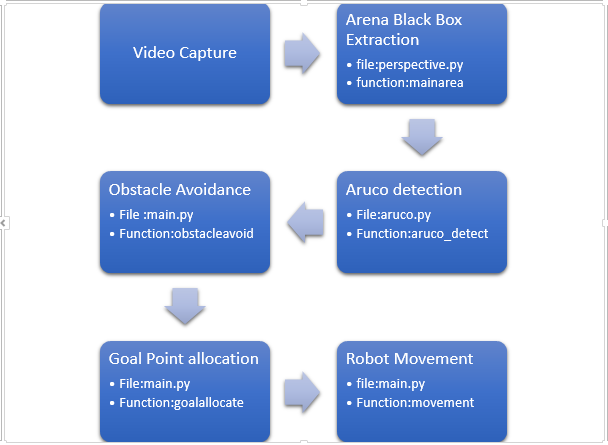
\includegraphics[scale=.8]{images/flowchart.png}

\pagebreak
\section{Video Capture}
To capture image using usb camera python uses a object created by the function cv2.VideoCapture('camera number'),
read() method of the cv2.VideoCapture(`camera number') is used to read single frame .
This full process is executed in a infinite while loop to process frame after frame and get a resulting video.
\begin{lstlisting}[language=Python, caption = Capturing Video]
		
cap=cv2.VideoCapture(1)
while(True):
	ret,frame=cap.read()
	cv2.imshow('window1',frame)
	k=cv2.waitKey(20) & 0xFF
	if k==27:
		cv2.destroyAllWindows()
       		 break	
'''cap is a object of cv2.VideoCapture'''
\end{lstlisting}

\section{Arena Black Box Extraction}
The main arena area is enclosed by a black boundary which can be extracted using the contour function.This function detects the shape with same color or intensity.

\begin{center}
	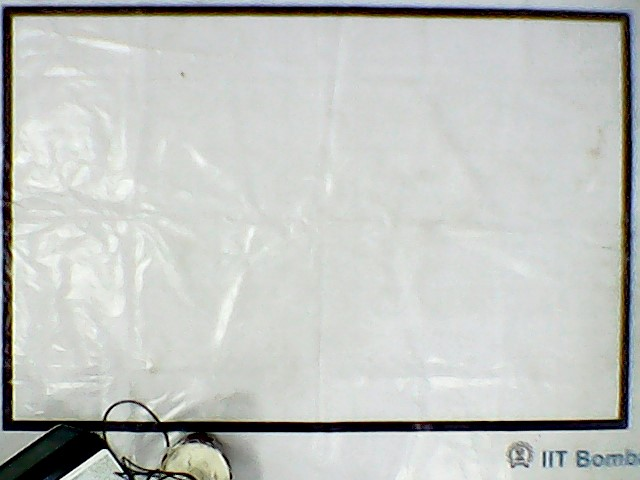
\includegraphics[scale=.6]{images/arena.jpg}
\end{center} 

\textbf{Steps:}
\begin{enumerate}
\item Convert the image into a grayscale image
\item Threshold the image
\item Apply the contour function
\item Loop over all the contours and find the desired contour by using functions like approxPolyDP or area
\item Perspective Transform
\end{enumerate}

\begin{lstlisting}[language=Python, caption = Black Box area crop and perspective trasform]
img_gray=cv2.cvtColor(img_rgb,cv2.COLOR_BGR2GRAY)
ret,thresh = cv2.threshold(img_gray,127,255,cv2.THRESH_BINARY)
_,contours,hierarchy=cv2.findContours(thresh,cv2.RETR_TREE,
cv2.CHAIN_APPROX_NONE)
for contour in contours:            
            approx = cv2.approxPolyDP(contour,0.01*cv2.arcLength(contour,True),True)
            area = cv2.contourArea(contour)        
            if (area >100000)and area<250000 :                
                x,y,w,h = cv2.boundingRect(contour)
                cv2.rectangle(img_rgb,(x,y),(x+w,y+h),(0,0,255),2)
pts1 = np.float32([[x,y],[x+w,y],[x,y+h],[x+w,y+h]])
pts2 = np.float32([[0,0],[w,0],[0,h],[w,h]])
M = cv2.getPerspectiveTransform(pts1,pts2)
arena = cv2.warpPerspective(crop_img,M,(w,h))
M = cv2.getPerspectiveTransform(pts1,pts2) 
dst = cv2.warpPerspective(img,M,(300,300))                
                
                
                
                
'''x,y are the coordinate of left top corner of the rectangle ,w and h are width and height of rectangle respectively,dst is the transformed image'''

\end{lstlisting}
\pagebreak	


\section{ArUco Detection} 
An ArUco marker is a synthetic square marker composed by a wide black border and a inner binary matrix which determines its identifier(id). The black border facilitates its fast detection in the image and the binary codification allows its identification and the application of error detection and correction techniques. The marker size determines the size of the internal matrix. For instance a marker size of 4x4 is composed by 16 bits.

ArUco marker pattern is based on hamming code where two column represents a data bit and three column represent parity bits.
Data bits when decoded gives the marker id whereas parity bits are useful in calculating the orientation and better detection of marker id.\\


\includegraphics[scale=.2]{images/aruco1.jpg}

\includegraphics[scale=.2]{images/aruco2.jpg}

\includegraphics[scale=.2]{images/aruco3.jpg}

\includegraphics[scale=.2]{images/aruco4.jpg}

ArUco detection is easily be done by using the arucodetectMarkers function 
of the opencv ArUco library. The function requires a grayscale image, aruco 
dictionary and the returned value from  detectorParameter\_create. detectParameter 
has data members such as thresholding, refinement, corner refinement etc to 
detect the ArUco from the image.
aruco.detectMarkers function returns the coordinates of the corners of the 
detected markers and their respective ids.
These corners are used to find the centroid and orientation of the aruco 
marker with respect to the horizontal axis in range -180 degrees to 180 
degrees.\\
A dictionary named robot is created having key as id of the marker 
containing items x and centroid and orientation angle of 
marker.\\
Vist the OpenCV ArUco docs for more information. \href{http://docs.opencv.org/3.1.0/d5/dae/tutorial_aruco_detection.html}{\ExternalLink}

\begin{center}
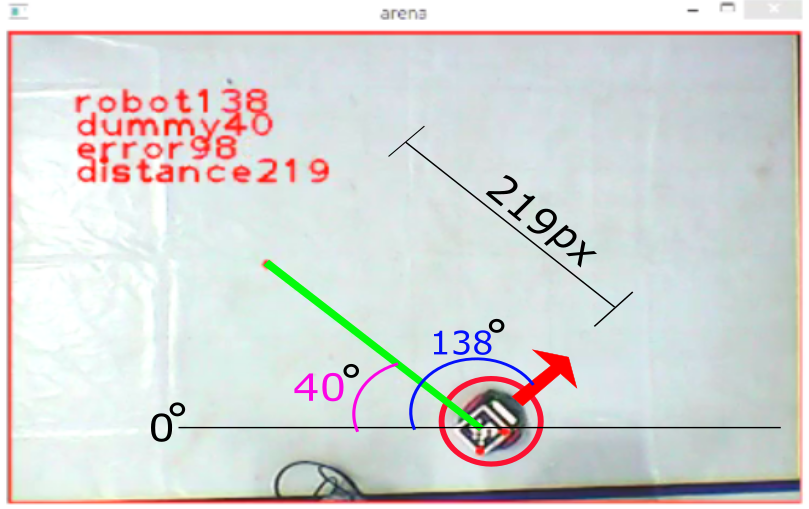
\includegraphics[scale=.5]{images/robot.png}
\end{center}

\begin{lstlisting}[language=Python, caption = Robot id as dictionary key with item centroid and angle]
gray = cv2.cvtColor(frame, cv2.COLOR_BGR2GRAY)
aruco_dict =aruco.Dictionary_get(aruco.DICT_5X5_250)
parameters = aruco.DetectorParameters_create()
corners,ids,_=aruco.detectMarkers(gray,aruco_dict,parameters=parameters)

for marker in range(len(ids)):
	x_center= int((corners[marker][0][0][0] + corners[marker][0][1][0] + corners[marker][0][2][0] + corners[marker][0][3][0])/4)
	y_center= int((corners[marker][0][0][1] + corners[marker][0][1][1] + corners[marker][0][2][1] + corners[marker][0][3][1])/4)
	cv2.circle(frame,(x_center,y_center),2,(0,0,255),2)
	x1 = int(corners[marker][0][0][0])
	x3 = int(corners[marker][0][3][0])
	y1 = int(corners[marker][0][0][1])
	y3 = int(corners[marker][0][3][1])           
	pt1=(x3,y3)
	pt2=(x1,y1)
	cv2.circle(frame,pt1,2,(0,0,255),2)
	cv2.circle(frame,pt2,2,(0,0,255),2)
	angle = angle_calculate(pt1,pt2)	robot[int(ids[marker])]=(int(x_center),int(y_center),int(angle))

print robot
\end{lstlisting}

\pagebreak	

\section{Collision Avoidance}

Since Atmega16 cannot handle data for all the robots in the arena therefore we need a collision avoidance check on the master which will only send a unique trigger command to the robot when its near collision. 

Collision avoidance requires two factors, relative angle and distance between the robots.

Algorithm Used for collision avoidance:
\begin{enumerate}

\item Calculate distance between robots.
\item Calculate Relative angle between robots.
\item Send command to the particular robot whose distance and relative angle are below threshold.
\end{enumerate}


Distance matrix: A distance matrix is a square matrix (two-dimensional array) containing the distances, taken pairwise, between the elements of a set.
\begin{lstlisting}[language=Python, caption = Distance Matrix ]

for i in robot:
	for j in robot:
	
		distancemat[i][j]=distance((robot[i[0],robot[i][1]),
		(robot[j][0],robot[j][1])) }
\end{lstlisting}
Angle Matrix: An angle matrix is a square matrix (two-dimensional array) containing the angle, taken pairwise, between the elements of a set. In this case angle is the relative angle that is angle of j with respect to i and vice- verse.

\begin{lstlisting}[language=Python, caption = Angle Matrix ]
for i in robot:
	for j in robot:
		obsy=(robot[j][1]-robot[i][1])
		obsx=(robot[j][0]-robot[i][0])
		angle_360=angle_calculate((robot[j][0],robot[j][1]),
			(robot[i][0],robot[i][1]))-robot[i][2] 
			#angle b/w robot i and robot j, with respect to angle of robot i (relative angle)       
		anglemat[i][j]=math.degrees(math.atan2(math.sin(angle_360*(math.pi/180)),math.cos(angle_360*(math.pi/180)))) #relative angle in range(-180 to 180) 
\end{lstlisting}

Apply a threshold on distance and angle to trigger robot to avoid collision.
np.where function of numpy is used to check the array and return the index of the element which is below the threshold value.

\begin{lstlisting}[language=Python, caption = Searching matrix ]
item=np.where(np.logical_and(distancemat[i][j]<80,distancemat[i][j]>0)) 
an=np.where(np.logical_and(anglemat[i][j]<90 , anglemat[i][j]>-90))
if (len(an[0])!=0)  and i!=j and len(item[0])!=0  : 
	obstacleavoid=True
\end{lstlisting}

\section{Goal Point allocation}
We use three ways to mark goal points on the canvas or image.
The three list goal, path, points are used to keep track of the points.

\begin{itemize}
	\item Goal-It contains the actual goal point for the robots.
	\item Path-It contains the possible goal points for all robots.
	\item Points-It contains raw points from the shape drawn on canvas.
\end{itemize}
The process of Goal allocation starts from points array if there exist one, then preferred points are transferred to the path array from where each robot chose its closes goal point and the chosen point is transferred to the goal array and becomes the true goal point for the particular robot.

\begin{enumerate}
\item Predefined points:

These points are directly defined in the array manually.

path= [(237, 160), (350, 179), (419, 132), (370, 69), (278, 79), (255, 273), (347, 296), (434, 279)]

\item One by one points:

To select points on image we use an opencv function 

cv2.setMouseCallback(`Window', function to call)
This function sets the handler for mouse activity calls the `function to call' when ever mouse is in the specified window.
\pagebreak
\begin{lstlisting}[language=Python, caption = Mouse activity call back function]
def draw_shape(event,x,y,flags,param):
    if event ==cv2.EVENT_RBUTTONDOWN:
    	''''Statement'''
    if event == cv2.EVENT_LBUTTONDOWN:
    	'''Statement'''
    elif  event == cv2.EVENT_MOUSEMOVE:
    	'''Statement'''            
    elif event == cv2.EVENT_LBUTTONUP:
    	'''Statement'''
        
\end{lstlisting}

\item single stroke shape:
\\
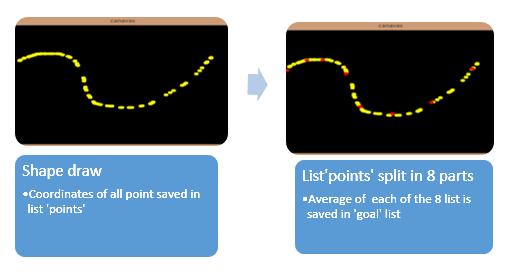
\includegraphics[scale=1]{images/shapedraw.png}
In this method all the points of the shape drawn on canvas are saved in the 'Points' array ,then the points are split into 8 parts maybe or may not be equal ,then average of each list is saved in 'path' array.

\begin{lstlisting}[language=Python, caption = Point selection from a shape]
This function takes an array and divides it into 8 parts
def chunkIt(seq, num):
  avg = len(seq) / float(num)
  out = []
  last = 0.0
  while last < len(seq):
    out.append(seq[int(last):int(last + avg)])
    last += avg
  return out

Averaging points in each list created by chunkIt function.
for i in range(len(chunk)):
	sumx=0
    sumy=0
    for j in (chunk[i]):       
    	sumx=(j[0]+sumx)
        sumy=(j[1]+sumy)
    tx=sumx/len(chunk[i])
    ty=sumy/len(chunk[i])
    path.append((tx,ty))
    return path
\end{lstlisting}


The final step is to move the points in path list to goal list. This is done by calculating distance between the robot and all the points in path list and chose the minimum distance point.

\begin{lstlisting}[language=Python, caption = Goal allocation]
initailly the Goal list is filled with (0,0)  
 for botid in robot:
        distance_list=[[]]
        for count,j in enumerate(path):            
            pt3=(robot[botid][0],robot[botid][1])
            pt4=j
            distance_list[count]=distance(pt3,pt4)
        goal_index=distance_list.index(min(distance_list))
        if (goal[botid]==(0,0)) and path!=[]:
            goal[botid]=path[goal_index]
            path.remove(goal[botid])
\end{lstlisting}
\end{enumerate} 

\section{Robot Movement}
To make the robot move for every frame a XBee packet is sent to bot containing its current robot id, location , orientation, its destination, angle of goal point , flag, rotation angle.
Flag and rotation are 0 in case of no obstacle avoidance mode and 1(left) or 2(right) in obstacle avoidance mode.
Similarly rotation angle is 0 for no obstacle avoidance mode and some integer for obstacle avoidance mode.

\pagebreak
\begin{lstlisting}[language=Python, caption = Robot Movement]
angle_dummy=angle_calculate(goal point,robot location)
'''here angle dummy is the angle of line between goal point robot location , w.r.t horizontal axis'''
        if obstacleavoid==False:
            if botid==0:
               xbees.tx(dest_addr='\x00\x20',
               data='<#'+str(i)+'/'+str(robot[i][0])+'/'+str(robot[i][1])+
               '/'+str(robot[i][2]+360)+
               '/'+str(dummy[0])+
               '/'+str(dummy[1])+
               '/'+str(angle_dummy+360+
               '/'+'0'+'0'+'/#>')
\end{lstlisting}

\section{Xbee Communication}
To enable serial communication we use a serial library of python.
It opens the COM port on which the XBee is connected and sets the baudrate for sending data.

In AT mode write method of 'serial' object can be used which does not create packets but sends the data serially character by character .


Xbee library of python is used when Xbee is configured in API mode.
The Xbee.tx function automatically create a acceptable packet for other xbees of a unique id (destination address) and the given data.
\begin{lstlisting}[language=Python, caption =Xbee API mode packet generation]

xbees.tx(dest_addr='\x00\x20',data='any string')

\end{lstlisting}





\pagebreak	

\end{document}